%--------------------------------------------------------------------%
%
% Title         : Postgraduate Thesis LaTex template
% Author        : Ravi Vendra Rishika <ravi.vendra.rishika@gmail.com>
%
% Page          : Chapter 2
%
% It is developed especially for postgraduate students of :
%   Department of Informatics
%   Faculty of Intelligent Electrical and Informatics Technology
%   Sepuluh Nopember Institute of Technology (ITS)
%   Surabaya, Indonesia.
%
% This LaTex template is intended to make students easier
% to write master's degree thesis in LaTex using specific
% Department of Informatics of ITS' format.
%
%--------------------------------------------------------------------%

\chapter{DASAR TEORI DAN TINJAUAN PUSTAKA}

Pada bab ini dijelaskan mengenai pustaka yang digunakan sebagai landasan ilmiah penelitian dan pustaka penelitian yang telah dilakukan sebelumnya terkait penelitian yang akan dilakukan.

\section{Kajian Pustaka}

\blindtext

\section{Dasar Teori}

Pada subbab ini akan dijelaskan seluruh teori berupa uraian kualitatif
maupun formula matematis dengan mengacu kepada kajian pustaka yang sudah digambarkan pada subbab sebelumnya.

\subsection{Dasar Teori ke-1}

\blindtext

\subsection{Dasar Teori ke-2}

\blindtext

\subsubsection{Dasar Teori ke-2.1}

\blindtext

\subsubsection{Dasar Teori ke-2.2}

\blindtext

\subsection{Dasar Teori ke-3}

\blindtext

\vspace{10pt}

\begin{figure}[h]
    \centering
    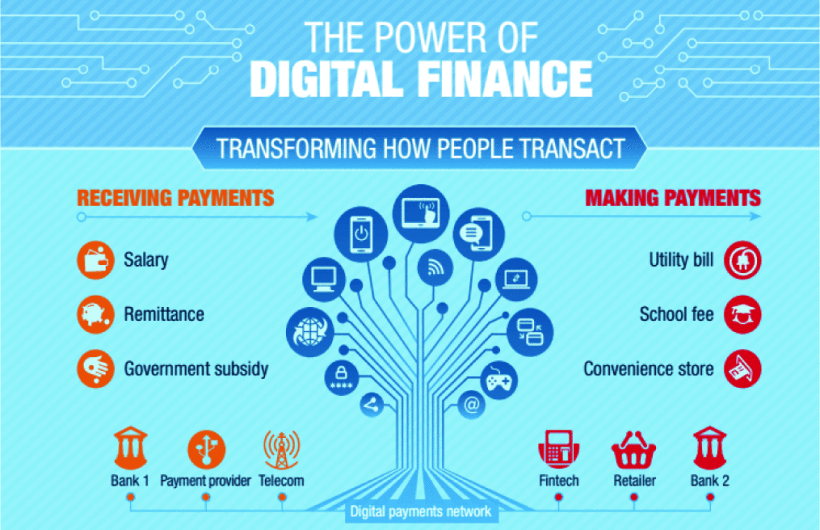
\includegraphics[width=0.90\textwidth]{src/resources/chapter-2-power-digital-finance.png}
    \caption{Transformasi Transaksi Finansial \textit{Fraud Detection System} \citep{8776857}}
    \label{fig:digital-finance}
\end{figure}

\vspace{10pt}

\subsection{Dasar Teori ke-4}

\blindtext

\blindtext
